\chapter{Linear Regression}

Regression is a fundamental concept that can modelling the relationship between a dependent variable and one or more independent variables. Linear regression is one of the simplest and most widely used regression techniques. It assumes a linear relationship between the input features and the output variable.

\section{Basic Concepts}

\subsection{Linear Model}

Traditional linear model can be represented as:
\[
y = w^T x + b
\]

where \(y\) is the predicted output, \(x\) is the input feature vector, \(w\) is the weight matrix, and \(b\) is the bias term.

More rigorously speaking, the formula above is a kind of \textbf{affine transformation}, which is a linear transformation followed by a translation. In this case, the linear transformation is represented by the weight matrix \(w\), and the translation is represented by the bias term \(b\).

\subsection{Loss Function}

The loss function quantifies the difference between the predicted output and the actual output. In linear regression, the most commonly used loss function is defined as:
\[
l^{(i)} = \frac{1}{2}(y^{(i)} - \hat{y}^{(i)})^2
\]

where \(l^{(i)}\) is the loss for the \(i\)-th training example, \(y^{(i)}\) is the actual output, and \(\hat{y}^{(i)}\) is the predicted output.

To measure the overall performance of the model on the entire training dataset, we can use the Mean Squared Error (MSE) loss function, which is defined as:
\[
L = \frac{1}{m} \sum_{i=1}^{m} l^{(i)} = \frac{1}{2m} \sum_{i=1}^{m} (y^{(i)} - \hat{y}^{(i)})^2
\]

where \(L\) is the overall loss, and \(m\) is the number of training examples.

The overall purpose is to find the optimal parameters \(w\) and \(b\) that minimize the loss function \(L\).

\subsection{Analytical Solution for Linear Regression}

Unlike other machine learning algorithms that require iterative optimization techniques, linear regression has a closed-form solution. The optimal parameters \(w\) and \(b\) can be computed directly using the following formulas:
\[
w = (X^T X)^{-1} X^T y
\]
\[
b = \bar{y} - w^T \bar{x}
\]

where \(X\) is the input feature matrix, \(y\) is the output vector, \(\bar{y}\) is the mean of the output values, and \(\bar{x}\) is the mean of the input features.

Analytical solution is computationally efficient for small to medium-sized datasets. However, for large datasets or high-dimensional feature spaces, iterative optimization techniques such as Gradient Descent are often preferred.

To better simulate the process of finding optimal parameters, we will introduce Gradient Descent in the next section.

\subsection{Random Gradient Descent}

Eventhough we have an analytical solution for linear regression, it is still beneficial to understand and implement Gradient Descent, as it is a widely used optimization technique in machine learning. In future cases, we will need to use Gradient Descent to optimize more complex models where analytical solutions are not feasible.

The simplest version of Gradient Descent is to calculate the loss function on the entire training dataset and update the parameters accordingly. This is known as Batch Gradient Descent. However, for large datasets, this approach can be computationally expensive. Instead, we can use minibatch stochastic gradient descent (SGD), which updates the parameters using a small random subset of the training data (minibatch) at each iteration.

The process can be expressed as follows:
\begin{enumerate}
    \item Randomly select a minibatch of training examples from the dataset.
    \item Compute the predicted outputs for the selected minibatch using the current parameters \(w\) and \(b\).
    \item Calculate the gradients of the loss function with respect to \(w\) and \(b\) using the selected minibatch.
    \item Update the parameters \(w\) and \(b\) using the computed gradients and a predefined learning rate \(\alpha\):
    \[
    w := w - \alpha \frac{\partial L}{\partial w} \quad
    b := b - \alpha \frac{\partial L}{\partial b}
    \]
    \item Repeat steps 1-4 for a predefined number of iterations or until convergence.
    \item Return the optimized parameters \(w\) and \(b\).
\end{enumerate}

Using minibatch SGD allows us to continuously convergent to the optimal parameters while reducing the computationally cost per iteration. But we can't actually guarantee that the parameters will converge to the exact optimal values as in the analytical solution. However, with a proper learning rate and sufficient iterations, we can achieve satisfactory results.

Linear regression with Gradient Descent provides a solid foundation for understanding optimization techniques in machine learning, which can be extended to more complex models in future chapters.

During the process, we recommend the reader to use \textbf{PyTorch} or \textbf{TensorFlow} to implement the algorithm, as these frameworks provide efficient tools for automatic differentiation and optimization.

\subsection{Normal Distribution and Linear Regression}

Now let's go back to the loss function we defined earlier:
\[
l^{(i)} = \frac{1}{2}(y^{(i)} - \hat{y}^{(i)})^2
\]
Why do we use this specific form of loss function in linear regression? The anser lies in the assumption that the errors (the differences between the actual outputs and the predicted outputs) follow a normal distribution, which is a common assumption in statistical modeling.

So first, let's take a look at what is a normal distribution.

\begin{definition}
    
A normal distribution is a continuous probability distribution characterized by its mean \(\mu\) and standard deviation \(\sigma\). The probability density function (PDF) of a normal distribution is given by:
\[
f(x) = \frac{1}{\sigma \sqrt{2\pi}} e^{-\frac{(x - \mu)^2}{2\sigma^2}}
\]

\end{definition}

\begin{definition}
In statistics, the likelihood function (often simply called the likelihood) measures the plausibility of a set of model parameters given some observed data. It is defined as the probability (or probability density) of observing the data, expressed as a function of the parameters.

Mathematically, if we have a set of observed data points \(D = \{x_1, x_2, \ldots, x_n\}\) and a statistical model with parameters \(\theta\), the likelihood function \(L(\theta; D)\) is given by:
\[
L(\theta; D) = P(D | \theta)
\]
\end{definition}

And our assumption can be written as:

\[
y = w^Tx + b + \epsilon, \quad \epsilon \sim \mathcal{N}(0, \sigma^2)
\]

where \(\epsilon\) represents the error term, which follows a normal distribution with mean 0 and variance \(\sigma^2\). Now we can derive the loss function from this assumption.

Given a training dataset with \(m\) examples, the likelihood function for the entire dataset can be expressed as the product of the individual likelihoods for each training example:
\[
L(w, b) = \prod_{i=1}^{m} P(y^{(i)} | x^{(i)}; w, b)
\]
Since the errors follow a normal distribution, we can express the conditional probability \(P(y^{(i)} | x^{(i)}; w, b)\) as:
\[
P(y^{(i)} | x^{(i)}; w, b) = \frac{1}{\sigma \sqrt{2\pi}} e^{-\frac{(y^{(i)} - (w^T x^{(i)} + b))^2}{2\sigma^2}}
\]
Substituting this into the likelihood function, we get:
\[
L(w, b) = \prod_{i=1}^{m} \frac{1}{\sigma \sqrt{2\pi}} e^{-\frac{(y^{(i)} - (w^T x^{(i)} + b))^2}{2\sigma^2}}
\]
To simplify the optimization process, we often work with the log-likelihood function instead of the likelihood function itself. Taking the natural logarithm of the likelihood function, we have:
\[
\ln L(w, b) = \sum_{i=1}^{m} \left( -\ln(\sigma \sqrt{2\pi}) - \frac{(y^{(i)} - (w^T x^{(i)} + b))^2}{2\sigma^2} \right)
\]
Maximizing the log-likelihood function is equivalent to minimizing the negative log-likelihood. Ignoring the constant term \(-\ln(\sigma \sqrt{2\pi})\), we can focus on minimizing the following expression:
\[
\sum_{i=1}^{m} \frac{(y^{(i)} - (w^T x^{(i)} + b))^2}{2\sigma^2}
\]
Since \(\sigma^2\) is a constant, minimizing this expression is equivalent to minimizing:
\[
\sum_{i=1}^{m} \frac{1}{2}(y^{(i)} - (w^T x^{(i)} + b))^2
\]
This is exactly the loss function we defined earlier for linear regression. Therefore, by assuming that the errors follow a normal distribution, we arrive at the conclusion that minimizing the Mean Squared Error (MSE) loss function is equivalent to maximizing the likelihood of the observed data given the model parameters.

\subsection{Neural Network Perspective}

All the content shown above can be easily extended to neural networks. In fact, a linear regression model can be seen as a simple neural network with no hidden layers and a linear activation function.

When we extend the linear model to a neural network, we introduce multiple layers of neurons, each with its own set of weights and biases. The output of each layer is passed through an activation function, which introduces non-linearity into the model. This allows the neural network to learn more complex relationships between the input features and the output variable.

We can express the neural network model as the following figure:

\begin{figure}[h]
    \centering
    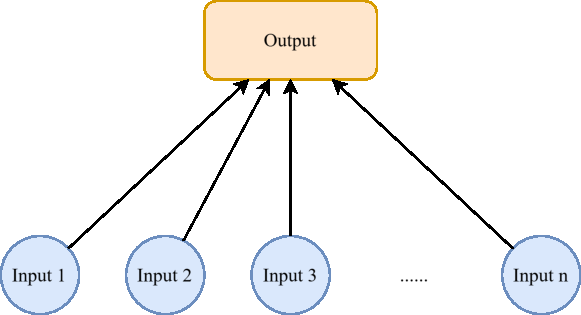
\includegraphics[width = 0.5\textwidth]{chapters/pics/insert_1_linear.pdf}
    \caption{Neural Network Perspective of Linear Regression}
\end{figure}

We can see that the linear regression model is equivalent to a neural network with a single neuron, where the weights and bias correspond to the parameters of the linear model. The loss function remains the same, as we still aim to minimize the Mean Squared Error (MSE) between the predicted outputs and the actual outputs.

For the neural network of linear regression, all the inputs are directly connected to the output neuron without any hidden layers. The output neuron performs a weighted sum of the inputs, adds a bias term, and produces the final output. We call this type of neural network a \textbf{fully-connected layer} or \textbf{dense layer}.

\subsubsection{Some Biology}

In biological neural networks, neurons are interconnected cells that transmit information through electrical and chemical signals. Each neuron consists of a cell body (soma), dendrites (input branches), and an axon (output branch). Dendrites receive signals from other neurons, which are then processed in the cell body. If the signal is strong enough, the neuron generates an action potential (electrical impulse) that travels down the axon to communicate with other neurons.

But nowadays, artificial neural networks are only loosely inspired by biological neural networks. While they share some similarities in terms of structure and function, artificial neural networks are simplified mathematical models that do not capture the full complexity of biological neurons, just like the Russell and Norvig said in their book \textit{Artificial Intelligence: A Modern Approach}.

What we have shown above is just a simple example of how linear regression can be viewed from a neural network perspective. As we delve deeper into the field of machine learning and neural networks, we will explore more complex architectures and techniques that build upon this foundational understanding.

\section{How to Achieve Linear Regression in Practice}

After we know the key idea of linear regression, we can implement it in practice using popular machine learning libraries \textbf{PyTorch}.

Here is a simple example of how to implement linear regression using PyTorch:

\begin{pythoncode}{Libraries}
import random
import torch
\end{pythoncode}

To make things simpler, we will generate some synthetic data for training the linear regression model.

\begin{pythoncode}{Data Generation}
# Generate synthetic data
def generate_data(w, b, num_examples):
    X = torch.normal(0, 1, (num_examples, len(w)))
    y = torch.matmul(X, w) + b
    y += torch.normal(0, 0.01, y.shape)
    return X, y.reshape((-1, 1))

true_w = torch.tensor([2.0, -3.4])
true_b = 4.2
features, labels = generate_data(true_w, true_b, 1000)
\end{pythoncode}

Now we can define the linear regression model using PyTorch's built-in modules. Have a review, we need to read the data, randomly select minibatches, define the model, define the loss function, and optimize the model parameters using Gradient Descent. Now we need to implement these steps in code.

\begin{pythoncode}{Random Minibatch Sampling}
# Define a function to get minibatches
def data_iter(batch_size, features, labels):
    num_examples = len(features)
    indices = list(range(num_examples))
    random.shuffle(indices)
    for i in range(0, num_examples, batch_size):
        batch_indices = torch.tensor(
            indices[i: min(i + batch_size, num_examples)])
        yield features[batch_indices], labels[batch_indices]
\end{pythoncode}

Why we use minibatches? Because using the entire dataset to compute the gradients can be computationally expensive, especially for large datasets. Minibatch SGD allows us to update the model parameters more frequently. Also, take advantage of the \textbf{GPU} acceleration, which can significantly speed up the training process.

Now let's define the linear regression model, first we need to initialize the model parameters (weights and bias):
\begin{pythoncode}{Model Definition}
w = torch.normal(0, 0.01, size=(2, 1), requires_grad=True)
b = torch.zeros(1, requires_grad=True)
\end{pythoncode}

Our next step is to construct the model's forward pass, which computes the predicted outputs given the input features, as well as defining the loss function and the optimization algorithm.

\begin{pythoncode}{Main Components}
# Define the linear regression model
def linreg(X, w, b):
    return torch.matmul(X, w) + b

# Define the Mean Squared Error loss function
def mse_loss(y_hat, y):
    return ((y_hat - y.reshape(y_hat.shape)) ** 2) / 2

# Define the SGD optimization algorithm
def sgd(params, lr, batch_size):
    with torch.no_grad():
        for param in params:
            param -= lr * param.grad / batch_size
            param.grad.zero_()
\end{pythoncode}

Now we can train the linear regression model using the defined components. We will iterate over the training data for a specified number of epochs, updating the model parameters using minibatch SGD.

\begin{pythoncode}{Training Loop}
# Training loop
lr = 0.03
num_epochs = 3
net = linreg
loss = mse_loss

# Main loop
for epoch in range(num_epochs):
    for X, y in data_iter(10, features, labels):
        l = loss(net(X, w, b), y)
        l.sum().backward()
        sgd([w, b], lr, batch_size=10)
    with torch.no_grad():
        train_l = loss(net(features, w, b), labels)
        print(f'epoch {epoch + 1}, loss {float(train_l.mean()):f}')
\end{pythoncode}

In the process of \texttt{l.sum().backward()}, PyTorch automatically computes the gradients of the loss with respect to the model parameters \(w\) and \(b\) using backpropagation. This is one of the key features of PyTorch that simplifies the implementation of machine learning algorithms.

After training the model, we can evaluate its performance by comparing the learned parameters \(w\) and \(b\) with the true parameters used to generate the synthetic data.

\begin{pythoncode}{Model Evaluation}
print(f'Learned weights: {w.reshape(true_w.shape)}')
print(f'Learned bias: {b}')
\end{pythoncode}

To summarize, we have implemented a linear regression model using PyTorch, demonstrating the key steps involved in training the model using minibatch stochastic gradient descent.

We can summarize it step by step as follows:
\begin{enumerate}
    \item Input the training data (features \(X\) and labels \(y\)).
    \item Forward pass: Compute the predicted outputs \(\hat{y}\) using the current model parameters \(w\) and \(b\).
    \item Loss computation: Calculate the loss \(L\) using the Mean Squared Error (MSE) loss function.
    \item Backward pass: Compute the gradients of the loss with respect to the model parameters \(w\) and \(b\) using backpropagation.
    \item Parameter update: Update the model parameters \(w\) and \(b\) using the computed gradients and the learning rate \(\alpha\) with the SGD optimization algorithm.
    \item Repeat steps 2-5 for a predefined number of epochs or until convergence.
\end{enumerate}

You can run the complete code in a Python enviroment with PyTorch installed to see the results. We provide the complete code in the folder for your convenience.

\section{How to Make Things Simpler}

We will introduce some predefined modules in PyTorch that can help us simplify the implementation of linear regression.

Just like what we have done before, we still need to define the model, loss function, and optimization algorithm. But this time, we can use PyTorch's built-in modules to simplify these steps.

Firstly, we still need to generate the synthetic data as before.

\begin{pythoncode}{Data Generation}
import random
import torch
from torch import nn

true_w = torch.tensor([2.0, -3.4])
true_b = 4.2
def generate_data(w, b, num_examples):
    X = torch.normal(0, 1, (num_examples, len(w)))
    y = torch.matmul(X, w) + b
    y += torch.normal(0, 0.01, y.shape)
    return X, y.reshape((-1, 1))

features, labels = generate_data(true_w, true_b, 1000)
\end{pythoncode}

Then, how can we read the data in minibatches? We can use PyTorch's built-in \texttt{DataLoader} module to handle the batching and shuffling of the data for us.

\begin{pythoncode}{DataLoader}
def load_array(data_arrays, batch_size, is_train=True):
    dataset = data.TensorDataset(*data_arrays)
    return data.DataLoader(dataset, batch_size, shuffle=is_train)

batch_size = 10
data_iter = load_array((features, labels), batch_size)
\end{pythoncode}

Next, we can define the linear regression model using PyTorch's \texttt{nn.Linear} module, which automatically handles the initialization of weights and biases for us.

\begin{pythoncode}{Model Definition}
# Define the linear regression model using nn.Linear
net = nn.Linear(2, 1)
\end{pythoncode}

Next, we can define the loss function using PyTorch's built-in \texttt{nn.MSELoss} module, which implements the Mean Squared Error loss function.
\begin{pythoncode}{Loss Function}
# Define the Mean Squared Error loss function using nn.MSELoss
loss = nn.MSELoss()
\end{pythoncode}

Finally, we can define the optimization algorithm using PyTorch's \texttt{torch.optim.SGD} module, which implements the Stochastic Gradient Descent optimization algorithm.
\begin{pythoncode}{Optimizer}
# Define the SGD optimization algorithm using torch.optim.SGD
trainer = torch.optim.SGD(net.parameters(), lr=0.03)
\end{pythoncode}

Now we can train the linear regression model using the defined components. The training loop remains similar to the previous implementation, but we can leverage the built-in modules to simplify the code.
\begin{pythoncode}{Training Loop}
# Training loop
num_epochs = 3
for epoch in range(num_epochs):
    for X, y in data_iter:
        l = loss(net(X), y)
        trainer.zero_grad()
        l.backward()
        trainer.step()
    l = loss(net(features), labels)
    print(f'epoch {epoch + 1}, loss {l:f}')
\end{pythoncode}

After training the model, we can evaluate its performance by comparing the learned parameters with the true parameters used to generate the synthetic data.

\begin{pythoncode}{Model Evaluation}
w = net.weight.data
b = net.bias.data
\end{pythoncode}

\section{Softmax Regression}

Softmax regression, also known as multinomial logistic regression, is an extension of linear regression that is used for multi-class classification problems. Unlike linear regression, which predicts continuous output values, softmax regression predicts the probabilities of each class for a given input.

\subsection{Model Definition}

The output of the softmax regression model is a probability distribution of each class. Considering a picture classification task with \(k\) classes, the output of the model is a \(k\)-dimensional vector, where each element represents the predicted probability of the input belonging to that class. The sum of all probabilities in the output vector is equal to 1.

So here comes the first question, how to choose the labels for multi-class classification? The answer is to use \textbf{one-hot encoding}.

\begin{definition}

One-hot encoding is a technique used to represent categorical variables as binary vectors. In one-hot encoding, each category is represented by a vector of length equal to the number of categories, where all elements are 0 except for the element corresponding to the category, which is set to 1.
\end{definition}

After defining the labels, we can define the softmax regression model. The model can be expressed as follows:
\[
o_1 = x_1 w_{11} + x_2 w_{12} + x_3 w_{13} + x_4 w_{14} + b_1
\]
\[
o_2 = x_1 w_{21} + x_2 w_{22} + x_3 w_{23} + x_4 w_{24} + b_2
\]
\[
o_3 = x_1 w_{31} + x_2 w_{32} + x_3 w_{33} + x_4 w_{34} + b_3
\]

where \(o_i\) is the output score for class \(i\), \(x_j\) is the input feature \(j\), \(w_{ij}\) is the weight connecting input feature \(j\) to class \(i\), and \(b_i\) is the bias term for class \(i\).

We can use a picture to illustrate the model structure:
\begin{figure}[h]
    \centering
    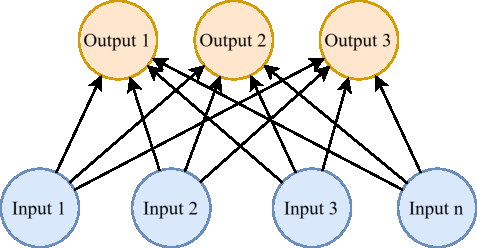
\includegraphics[width = 0.5\textwidth]{chapters/pics/insert_2_softmax.pdf}
    \caption{Softmax Regression Model Structure}
\end{figure}

\newpage

Now we have the output scores for each class, but we need to convert these scores into probabilities. This is where the softmax function comes into play.

We cannot directly use the output scores for classification, as they can be any real number and do not represent probabilities. The softmax function transforms the output scores into probabilities by applying the following formula:

\[
P(y = i | x) = \frac{e^{o_i}}{\sum_{j=1}^{k} e^{o_j}}
\]

where \(P(y = i | x)\) is the predicted probability of class \(i\) given input \(x\), \(o_i\) is the output score for class \(i\), and \(k\) is the total number of classes.

Althougn the softmax function is not linear, the model is still called softmax regression because the output scores \(o_i\) are computed using a linear combination of the input features. Thus, softmax regression can be seen as a linear model followed by a non-linear activation function (softmax) to produce probabilities.

We also need to define the loss function for softmax regression. The most commonly used loss function for multi-class classification is the Cross-Entropy Loss, which measures the difference between the predicted probability distribution and the true distribution (one-hot encoded labels).

The Cross-Entropy Loss can be expressed as follows:
\[
L = -\sum_{i=1}^{k} y_i \ln(P(y = i | x))
\]

We can derive the loss function from the likelihood function, just like what we have done in linear regression. Given a training dataset with \(m\) examples, the likelihood function for the entire dataset can be expressed as the product of the individual likelihoods for each training example:
\[
L(w, b) = \prod_{i=1}^{m} P(y^{(i)} | x^{(i)}; w, b)
\]
Taking the natural logarithm of the likelihood function, we have:
\[
\ln L(w, b) = \sum_{i=1}^{m} \ln(P(y^{(i)} | x^{(i)}; w, b))
\]
Maximizing the log-likelihood function is equivalent to minimizing the negative log-likelihood. Ignoring the constant terms, we can focus on minimizing the following expression:
\[
-\sum_{i=1}^{m} \sum_{j=1}^{k} y_j^{(i)} \ln(P(y = j | x^{(i)}; w, b))
\]
This is exactly the Cross-Entropy Loss function we defined earlier for softmax regression. Therefore, by maximizing the likelihood of the observed data given the model parameters, we arrive at the conclusion that minimizing the Cross-Entropy Loss function is equivalent to maximizing the likelihood.

For how to derive the Cross-Entropy Loss function in detail, please refer to the content about \textbf{Information Theory} on the internet.

\newpage

\subsection{MNIST}

The MNIST dataset is a widely used benchmark dataset for image classification tasks, particularly for handwritten digit recognition. It consists of 60,000 training images and 10,000 test images of handwritten digits (0-9), each represented as a 28x28 grayscale image.

In this section, we will implement softmax regression using PyTorch to classify the Fashion-MNIST dataset. We will follow similar steps as in the previous linear regression example, but with modifications to accommodate the multi-class classification task.

\begin{pythoncode}{Libraries}
import torch
import torchvision
from torch.utils import data
from torchvision import transforms
\end{pythoncode}

Now we will load the Fashion-MNIST dataset using PyTorch's \texttt{torchvision} module. We will apply necessary transformations to the images, such as converting them to tensors and normalizing the pixel values.

\begin{pythoncode}{Data Loading}
# Load the Fashion-MNIST dataset
trans = transforms.ToTensor()
mnist_train = torchvision.datasets.FashionMNIST(
    root="../data", train=True, transform=trans, download=True)
mnist_test = torchvision.datasets.FashionMNIST(
    root="../data", train=False, transform=trans, download=True)
\end{pythoncode}

As we have already known, the \textbf{Fashion-MNIST} dataset contains 10 classes of clothing items, including T-shirts, trousers, pullovers, dresses, coats, sandals, shirts, sneakers, bags, and ankle boots. Each image is a 28x28 grayscale image, which we will flatten into a 784-dimensional vector for input to the softmax regression model.

Now let's define the data loader to read the data in minibatches.

\begin{pythoncode}{DataLoader}
batch_size = 256
train_iter = data.DataLoader(mnist_train, batch_size, shuffle=True, num_workers=4)
\end{pythoncode}

Now we can define the function \texttt{load\_data\_fashion\_mnist} to encapsulate the data loading process for convenience.

\begin{pythoncode}{Data Loading Function}
def load_data_fashion_mnist(batch_size, resize=None):
    trans = [transforms.ToTensor()]
    if resize:
        trans.insert(0, transforms.Resize(resize))
    trans = transforms.Compose(trans)
    mnist_train = torchvision.datasets.FashionMNIST(
        root="../data", train=True, transform=trans, download=True)
    mnist_test = torchvision.datasets.FashionMNIST(
        root="../data", train=False, transform=trans, download=True)
    return (data.DataLoader(mnist_train, batch_size, shuffle=True,
                            num_workers=get_dataloader_workers()),
            data.DataLoader(mnist_test, batch_size, shuffle=False,
                            num_workers=get_dataloader_workers()))
\end{pythoncode}

The parameter "resize" allows us to resize the images if needed. The function returns the training and test data loaders.

Now we can define the softmax regression model using PyTorch's \texttt{nn.Linear} module, which automatically handles the initialization of weights and biases for us.

Firstly let's initialize the model parameters (weights and bias):

\begin{pythoncode}{Model Definition}
num_inputs = 784
num_outputs = 10

W = torch.normal(0, 0.01, size=(num_inputs, num_outputs), requires_grad=True)
b = torch.zeros(num_outputs, requires_grad=True)
\end{pythoncode}

Then we can define the softmax regression model, loss function, and optimization algorithm.

\begin{pythoncode}{Main Components}
# Define the softmax regression model
def softmax(X):
    X_exp = torch.exp(X)
    partition = X_exp.sum(1, keepdim=True)
    return X_exp / partition
\end{pythoncode}

During the process of calculating the softmax function, we use the \texttt{keepdim=True} parameter to ensure that the output tensor maintains the same number of dimensions as the input tensor. This is important for subsequent operations, such as loss calculation, where we need to align the dimensions of the predicted probabilities and the true labels. Also, we use the \textbf{broadcasting} feature of PyTorch to perform element-wise division between the exponentiated scores and the partition function.

\begin{pythoncode}{Loss Function and Optimizer}
# Define the cross-entropy loss function
def net(X):
    return softmax(torch.matmul(X.reshape((-1, W.shape[0])), W) + b)

# Define the cross-entropy loss function
def cross_entropy(y_hat, y):
    return -torch.log(y_hat[range(len(y_hat)), y])
\end{pythoncode}

Instead of computing the loss using the full formula that sums over all classes, this implementation uses an efficient indexing trick. The expression \texttt{y\_hat[range(len(y\_hat)), y]} performs advanced indexing:

\begin{enumerate}
    \item For each sample in the batch, it selects the predicted probability corresponding to the true class label \(y\).
    \item This results in a 1-dimensional tensor containing the predicted probabilities for the correct classes for all samples in the batch.
    \item Finally, the negative logarithm of these probabilities is computed to obtain the cross-entropy loss for each sample.
\end{enumerate}

It is logically equivalent to the function below:

\begin{pythoncode}

def cross_entropy_onehot(y_hat, y):
    y_onehot = torch.zeros_like(y_hat)
    y_onehot[range(len(y_hat)), y] = 1
    return -(y_onehot * torch.log(y_hat)).sum(dim=1)
\end{pythoncode}

But the first implementation is more efficient in terms of computation and memory usage.

Afterall, we have defined the loss function. However, in real life applications, we need to output the predicted class labels based on the predicted probabilities. This can be achieved using the \texttt{argmax} function, which returns the index of the maximum value along a specified dimension.

\begin{pythoncode}{Prediction Function}
def accuracy(y_hat, y):
    if len(y_hat.shape) > 1 and y_hat.shape[1] > 1:
        y_hat = y_hat.argmax(axis=1)
    cmp = y_hat.type(y.dtype) == y
    return float(cmp.type(y.dtype).sum())
\end{pythoncode}

Here we define a class \texttt{Accumulator} to help us accumulate the sum of multiple variables over time, which is useful for tracking metrics like loss and accuracy during training.

\begin{pythoncode}{Accumulator Class}
class Accumulator:
    def __init__(self, n):
        self.data = [0.0] * n

    def add(self, *args):
        self.data = [a + float(b) for a, b in zip(self.data, args)]

    def reset(self):
        self.data = [0.0] * len(self.data)

    def __getitem__(self, idx):
        return self.data[idx]
\end{pythoncode}

Finally, we can define the training function to encapsulate the training process for convenience.

\begin{pythoncode}{Training Function}
def train_epoch_ch3(net, train_iter, loss, updater):
    if isinstance(net, torch.nn.Module):
        net.train()
    metric = Accumulator(3)
    for X, y in train_iter:
        y_hat = net(X)
        l = loss(y_hat, y).sum()
        if isinstance(updater, torch.optim.Optimizer):
            updater.zero_grad()
            l.backward()
            updater.step()
        else:
            l.backward()
            updater(X.shape[0])
        metric.add(float(l), accuracy(y_hat, y), y.numel())
    return metric[0] / metric[2], metric[1] / metric[2]
\end{pythoncode}

The training function defined above trains the model for only one epoch. To evaluate the model's performance on the test dataset, we need a function to compute the accuracy on the test set.

\begin{pythoncode}{Evaluation Function}
def evaluate_accuracy(net, data_iter):
    if isinstance(net, torch.nn.Module):
        net.eval()
    metric = Accumulator(2)
    with torch.no_grad():
        for X, y in data_iter:
            metric.add(accuracy(net(X), y), y.numel())
    return metric[0] / metric[1]
\end{pythoncode}

Now we can combine everything to define the complete training loop, which iterates through multiple epochs, trains the model, and evaluates its performance on the test dataset at the end of each epoch.

\begin{pythoncode}{Complete Training Loop}
def train_ch3(net, train_iter, test_iter, loss, num_epochs, updater):
    for epoch in range(num_epochs):
        train_metrics = train_epoch_ch3(net, train_iter, loss, updater)
        test_acc = evaluate_accuracy(net, test_iter)
        print(f'epoch {epoch + 1}, loss {train_metrics[0]:.4f}, '
              f'train acc {train_metrics[1]:.3f}, test acc {test_acc:.3f}')
\end{pythoncode}

With all the components in place, we can now train the model.

\begin{pythoncode}{Run Training}
num_epochs = 10
lr = 0.1

def updater(batch_size):
    return torch.optim.SGD([W, b], lr=lr)

train_ch3(net, train_iter, mnist_test, cross_entropy, num_epochs, updater)
\end{pythoncode}

Before making predictions, we need to define some helper functions to visualize the images and labels. We also need to import \texttt{matplotlib.pyplot}.

\begin{pythoncode}{Visualization Helpers}
import matplotlib.pyplot as plt

def get_fashion_mnist_labels(labels):
    text_labels = ['t-shirt', 'trouser', 'pullover', 'dress', 'coat',
                   'sandal', 'shirt', 'sneaker', 'bag', 'ankle boot']
    return [text_labels[int(i)] for i in labels]

def show_images(imgs, num_rows, num_cols, titles=None, scale=1.5):
    figsize = (num_cols * scale, num_rows * scale)
    _, axes = plt.subplots(num_rows, num_cols, figsize=figsize)
    axes = axes.flatten()
    for i, (ax, img) in enumerate(zip(axes, imgs)):
        if torch.is_tensor(img):
            ax.imshow(img.numpy())
        else:
            ax.imshow(img)
        ax.axes.get_xaxis().set_visible(False)
        ax.axes.get_yaxis().set_visible(False)
        if titles:
            ax.set_title(titles[i])
    return axes
\end{pythoncode}

After training, we can use the trained model to make predictions on some images from the test dataset.

\begin{pythoncode}{Prediction}
def predict_ch3(net, test_iter, n=6):
    for X, y in test_iter:
        break
    trues = get_fashion_mnist_labels(y)
    preds = get_fashion_mnist_labels(net(X).argmax(axis=1))
    titles = [true +'\n' + pred for true, pred in zip(trues, preds)]
    show_images(X[0:n].reshape((n, 28, 28)), 1, n, titles=titles[0:n])

predict_ch3(net, mnist_test)
\end{pythoncode}

This concludes the implementation of Softmax Regression using PyTorch. The model is now capable of classifying images from the Fashion-MNIST dataset with reasonable accuracy.

You can run the complete code in a Python enviroment with PyTorch and torchvision installed to see the results. We provide the complete code in the folder for your convenience.

Now you have learned how to implement both Linear Regression and Softmax Regression using PyTorch. These foundational techniques are essential for understanding more complex machine learning models and algorithms that will be covered in later chapters.

In the next chapter, we will explore a real neural network architecture called \textbf{Multilayer Perceptron (MLP)}, which builds upon the concepts learned in this chapter and introduces additional layers and non-linear activation functions to enhance the model's capacity to learn complex patterns in data.
